
%\nipsfinalcopy % Uncomment for camera-ready version

\subsection{Notation}

Unless otherwise specified, we let lower-case English alphabet characters indicate scalars $x \in \Real$, bold indicates column vectors $\mb{x} \in \Real^p$, and upper-case bold indicates matrices, $\bX \in \Real^{p \times q}$.  Parameters and constants will be Greek characters.  Time will be $t \in (0,T)$, $i \in [N]$ will index the $N$ neurons, where $[N]=\{1,2,\ldots,N\}$. Script will denote sets and pipes will denote the cardinality of the set, e.g. $|\mc{T}|$.  

\subsection{Input}
% \subsection{Data Model}
Our data is a time-series of multielectrode recordings $\bX \equiv (\bx_1, \cdots, \bx_T)$, and consists of $T$ recordings from $C$ channels. 
The set of recording times lie on regular grid with interval length $\Delta$, while $\bx_t \in \mathbb{R}^C$ for all $t$. 
This time-series of electrical activity is driven by an unknown number of neurons {\color{red} and we want to... recap scientific goals}. 
We let the number of neurons be unbounded, though only a few of the infinite
neurons dominate. These neurons contribute the majority of the activity in any finite interval of time; however, as time passes, the total number of 
observed neurons increases {\color{red}(Justify?)}. 
%Each neuron, has its own `shape' A natural model in such a situation is to
The neurons themselves generate continuous-time voltage traces, with the outputs of all neurons superimposed and discretely sampled to produce the 
recordings $\bX$.  At a high level, we model the output of each neuron as a
series of idealized spikes which are smoothed with appropriate kernels, the latter determining the shape of each spike. 
%Each neuron has its own distribution over waveform shapes. 
We describe this in detail, starting first with a model for a single channel recording $\bx\T \equiv (x_1, \cdots, x_T)$.

\subsection{Modeling a single electrode recording}

There is a rich literature characterizing the spiking activity of a single neuron \citep{}, accounting in detail for factors like non-stationarity, 
refractoriness and spike waveform. We shall however make a number of simplifying assumptions (some of which we later relax, others we expect to relax in future work). Figure \ref{fig:schematic} provides a schematic depiction of our generative process.
First, we model the spiking activity of each neuron is 
stationary and memoryless, so that its set of spike times are 
distributed as a homogeneous Poisson process. 
{\color{red} justify?} We model the neurons themselves are heterogeneous, with the $i^{th}$ neuron having
an (unknown) firing rate $\lambda_i$. Call the ordered set of spike times of the $i^{th}$ neuron $\mc{T}_i$; then the time between successive elements of $\mc{T}_i$ is 
exponentially distributed with mean $1/\lambda_i$. We write this as
\begin{align}
  \mc{T}_i &\sim \text{PoissProc}(\lambda_i)
\end{align}
The actual electrical output of a neuron is not binary; instead each spiking event is a smooth perturbation in voltage about a
resting state. This perturbation forms the shape of the spike, and without any loss of generality, we set the resting state to zero. 
{(\color{red} figure? better biological description? comment on how we preprocess the data to get zero mean?)}. 
While the spike shapes vary across neurons as well as across different spikes of the same neuron, each 
neuron has its own characteristic distribution over shapes. 
We let $\bth^*_i \in \Theta$ parametrize this distribution for neuron $i$.
 % having parameter $\bth^*_i$. 
Whenever this neuron emits a 
spike, a new shape is drawn independently from the corresponding distribution. %$p_{\bth_i}$, and 
This waveform is then offset to the time of the spike, and contributes to the voltage trace associate with that spike. The complete detected output of the neuron is the 
superposition of all these spike waveforms plus noise.  
We assume the noise is independent and  identically distributed Gaussian noise at each time step.

% Comment on how this dictionary is obtained now, or in section on inference?)}. 
We model the random spike shapes themselves as weighted superpositions of a dictionary of $K$ basis functions $\bd(t) \equiv (d_1(t), \cdots, d_K(t))\T$. The
dictionary elements are shared across all neurons, and each is a real-valued function of time, e.g., $d_k \in L_2$.
For the $i^{th}$ neuron, the $j^{th}$ spike $\tau_{ij} \in \mc{T}_i$, is associated with a random $K$-dimensional weight vector $\tby_{ij} \equiv (\ty_{ij1}, \ldots \ty_{ijK})\T$, and the 
shape of this spike is given by the weighted sum $\sum_{k=1}^K \ty_{ijk} d_k(t)$. We assume $\tby_{ij} \sim \mc{N}_K(\mb{\mu}^*_i, \Sigma^*_i)$ indicating a $K$-dimensional Gaussian distribution with mean $\mb{\mu}^*_i$ and covariance $\Sigma^*_i$.   Then, at any time $t$, the output of neuron $i$ is
\begin{align}
  x_{i}(t) &= \sum_{j=1}^{|\mc{T}_i|} \sum_{k=1}^K \ty_{ijk} d_k(t - \tau_{ij})
\end{align}



% \begin{center}
% \begin{figure}
% % 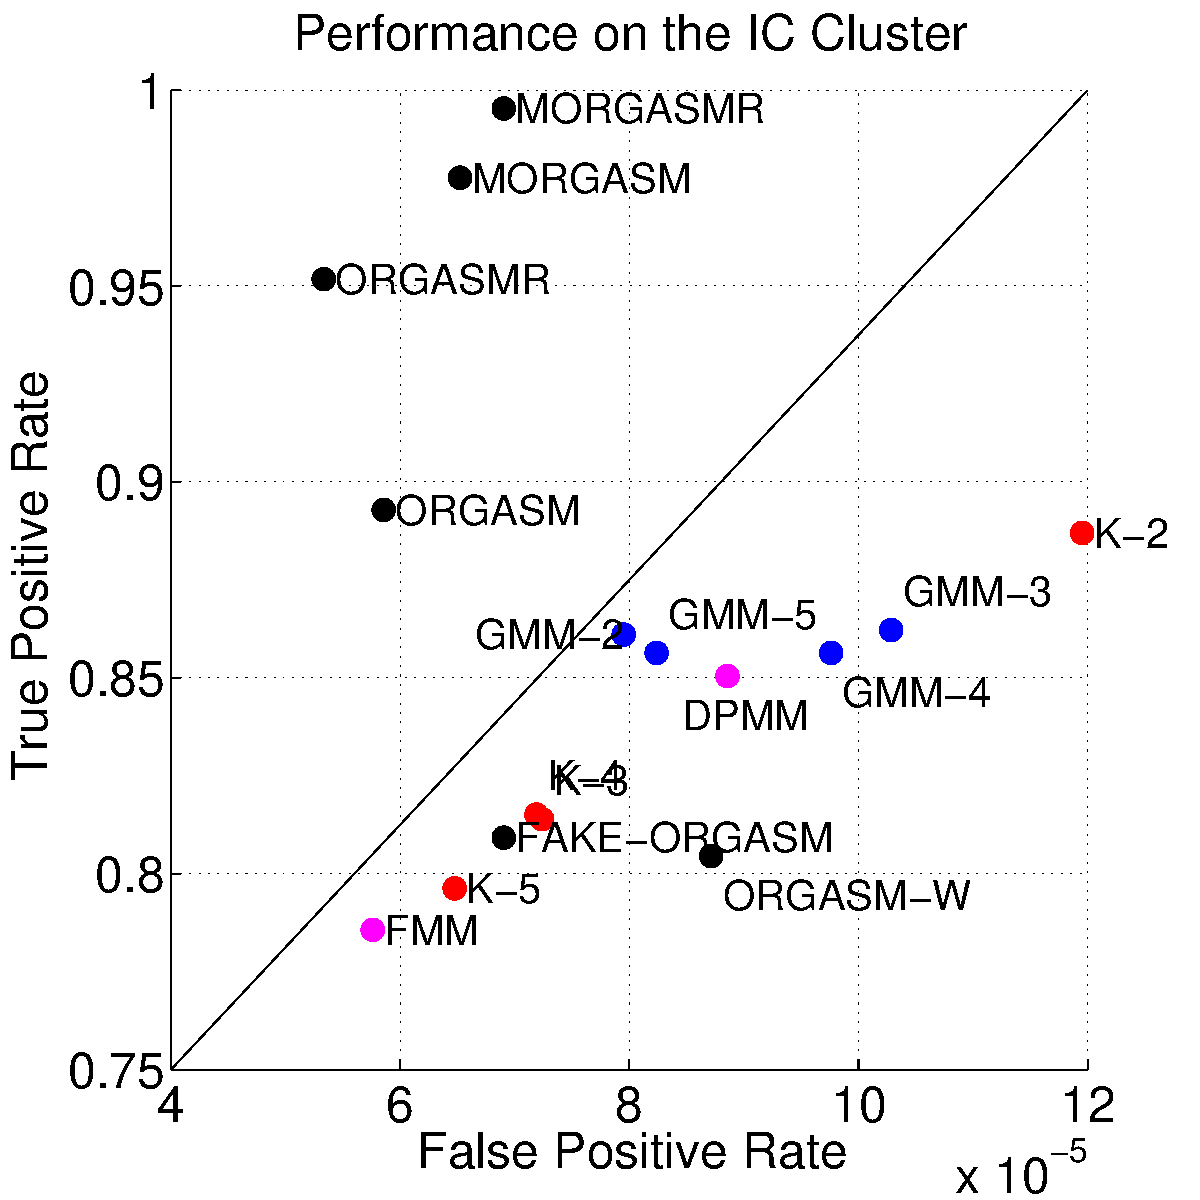
\includegraphics[width=\textwidth]{../figs/truefalsepositive}
% \caption{Schematic of our Generative Model.}
% \label{fig:schmetic}
% \end{figure}
% \end{center}

{The total signal recorded from any electrode  is the superposition of the outputs of all neurons. Assume for the moment there are $N$
neurons, and define $\mc{T} = \cup_{i \in [N]} \mc{T}_i$ as
the (ordered) union of the spike times of all neurons. 
Let $\tau_l$ indicate the $l^{th}$ overall spike, that is $\tau_l \in \mc{T}$, whereas $\tau_{ij} \in \mc{T}_i$ is the $j^{th}$ spike of neuron $i$.
To map elements  $\tau_{ij} \in \mc{T}_i$ to elements  $\tau_l \in \mc{T}$,   we implicitly have defined a mapping from $(N \times |\mc{T}_i|)$ to $|\mc{T}|$. %, which maps from the $j^{th}$ spikes of neuron $i$ to the $l^{th}$ overall spike.

Let $\nu_l \in N$ be the neuron to which the $l^{th}$ element of $\mc{T}$ belongs, 
and let $\bth_l \equiv (\mb{\mu}_l, \Sigma_l)$ be the neuron parameter associated with
that spike. 
Thus $\bth_l = \bth^*_{\nu_l}$. 
% Furthermore, let $p_j \from \mc{T} \to \mc{T}_j$ index the position of spike $j$ of $\mc{T}$ in $\mc{T}_{\nu_j}$.
% , the spike train of neuron $\nu_j$. 
Thus $\tau_l = \tau_{\nu_l j}$ is the $j^{th}$ spike of neuron $\nu_l$. Finally, define $\by_l=(y_{l1}, \ldots, y_{lK})\T \equiv \tby_{\nu_j j}$ as the weight vector of spike $\tau_l$. Then, we have that}
\begin{subequations}
\begin{align}
  x(t) &= \sum_{i \in [N]} x_{i}(t) =   \sum_{l \in |\mc{T}|} \sum_{k \in [K]} y_{lk} d_k(t - \tau_{l}),  \label{eq:spk_sup} \\
% \intertext{where}
  \by_{l} & \sim \mc{N}_K(\mb{\mu}_{l}, \Sigma_{l}). \label{eq:spk_shape}
\end{align}
\end{subequations}
% 
From the superposition property of the Poisson process \citep{kingman93}, the overall spiking activity $\mc{T}$ is a 
Poisson process with rate $\Lambda = \sum_{i \in [N]} \lambda_i$. Each event $\tau_l \in \mc{T}$ is associated with a pair of labels, the parameter of the neuron to which it 
is assigned ($\bth_l = (\mb{\mu}_l, \Sigma_l)$), and the weight-vector characterizing the spike shape ($\by_l$). We can view these as the ``marks'' of a 
marked Poisson process $\mc{T}$.  From the properties of the Poisson process, we have that the marks $\bth_l$ are drawn i.i.d. from a probability measure 
\begin{align}
 G(\dd \bth) = \frac{1}{\Lambda}\sum_{i \in [N]} \lambda_i \delta_{\bth^*_i}    \label{eq:mark_distr}
\end{align}
Note that with probability one, the neurons have distinct parameters, so that the mark $\bth_l$ associated with spike $l$ identifies the
neuron which produced it: $G(\bth_l = \bth^*_i) = P(\nu_l= i) = \lambda_i/\Lambda$. Given $\bth_l$, $\by_l$ is distributed as in
Eq.~\eqref{eq:spk_shape}. The output waveform $x(t)$ is then a linear functional of this marked Poisson process (Eq.~\eqref{eq:spk_sup}). 

\subsection{Completely random measures (CRMs)}

The previous section assumed a known number of neurons $N$. In practice however, our recordings are a superposition of the outputs of an unknown
number of neurons. We deal with this uncertainty by taking a nonparametric Bayesian approach, and letting the number of neurons $N$ tend to infinity
{\color{red} Can we provide a biological/electrical justification of this?}. 
Such an approach leads to an elegant and flexible modeling framework, and has  already proved successful in neuroscience applications
\citep{WoodBla2008}.
Since only a finite number of spikes are observed in any finite interval, the total rate $\Lambda$ must 
also be finite; moreover, as we described earlier, we want this to be dominated by a few $\lambda_i$. 
A natural framework that captures these  modeling requirements is that of completely random measures \citep{Kingman:PJM67}.
Completely random measures are stochastic processes that form flexible and convenient priors over
infinite dimensional objects like probability distributions \citep{JamesLP09}, hazard functions \citep{Hjo1990}, latent features \citep{ThiJor2007} etc. 
These have been well studied in the Bayesian nonparametrics and machine learning communities, and there exists a wealth of literature on
their theoretical properties, as well as on computational approaches to posterior inference.

Recall that each neuron is characterized by a pair of parameters $(\lambda_i, \bth^*_i)$; the former characterizes the distribution over spike times, 
and the latter over spike
shapes. With Eq.~\eqref{eq:mark_distr} in mind, we map the infinite collection of pairs $\{(\lambda_i, \bth^*_i)\}$ to an atomic measure on $\Theta$:
\begin{align}
  \Lambda(\dd \bth) = \sum_{i=1}^{\infty} \lambda_i \delta_{\bth^*_i}
\end{align}
For any subset $\varTheta$ of $\Theta$, the measure $\Lambda(\varTheta)$ equals \( \sum_{\{ i: \bth^*_i \in \varTheta \} } \lambda_i\). We allow $\Lambda(\cdot)$ to be random,
modeling it as a realization of a completely random measure. Such a random measure has the property that for any two disjoint subsets $\varTheta_1$,  $\varTheta_2 \subseteq \Theta$, the measures $\Lambda(\varTheta_1)$ and $\Lambda(\varTheta_2)$ are independent. 
This distribution over measures is induced by a distribution
over the infinite sequence of weights (the $\lambda_i$'s), and a distribution over the sequence of their locations (the $\bth^*_i$'s). 
For a CRM, the weights $\lambda_i$ are the jumps of a \Levy process \citep{Sato90}, and their distribution is characterized by a 
\Levy measure $\rho(r)$. The locations $\bth^*_i$ are drawn i.i.d.\  from a base probability measure $H(\bth^*)$.
As is typical, we assume these to be independent (though this is not necessary). {\color{red} if there's space, I
can elaborate on the construction of the CRM from its Levy measure, though this is not necessary}

The particular class of CRM is determined by the \Levy measure $\rho(r)$. For our application, we set $\rho(r) = r^{-1}\exp(-r\alpha)$;
this results in a CRM called the Gamma process ($\Gamma$P) \citep{applebaum2004}. 
The Gamma process has the convenient property that the 
total rate $\Lambda \equiv \Lambda(\Theta) = \sum_{i=1}^{\infty} \lambda_i$ is Gamma distributed (and thus conjugate to the Poisson process prior on $\mc{T}$).
%\footnote{We abuse notation by using $\Lambda$ to denote both the measure as well as the total measure of $\Theta}
%The Gamma distribution has shape parameter $1$ and scale parameter $\alpha$.  Since this is finite almost surely, so too is $\mc{T}$. 
The Gamma process is also closely connected with the Dirichlet process \citep{Ferguson73}, which will prove useful
later on.
Other choices of the \Levy intensity can be used to capture greater uncertainty in the number of neurons active in any finite interval, or to model
power-law behavior in the number of spikes emitted by different neurons.

To complete the specification on the Gamma process, we need to choose a base-measure $H(\bth^*)$.
Recalling that $\bth^* \equiv (\mu^*, \Sigma^*)$ gives the mean and variance of the weight-vector $\by$ of each neuron, we set $H(\bth^*)$ 
to be the conjugate normal-Wishart distribution. Our overall model is then:
\begin{subequations}
\begin{align}
  \Lambda(\cdot) & \sim \Gamma \text{P}(\alpha, H(\cdot)) \\ %\mathcal{NW}(\mu, \Sigma)) \\
  \mc{T}_i\ \  &\sim \text{PoissProc}(\lambda_i) \quad i \in \ZZ \\
  \by_{ij} & \sim \mc{N}_K(\mb{\mu}^*_i, \Sigma^*_i) \quad i,j \in \ZZ \\
  x_i(t) &= \sum_{j = 1}^{|\mc{T}_i|}  \sum_{k = 1}^{K} \tilde{y}_{ijk} d_k(t - \tau_{ij}) \\
  x(t)   &= \sum_{i=1}^{\infty} x_i(t)
\end{align}
\end{subequations}
%Each spike of each neuron is associated with a time $e$ and a weight vector $y$, and one can view the model above as a doubly stochastic Poisson
%process on the product space. 
% 
It will be more convenient to work with the marked Poisson process representation of Eqs.~\eqref{eq:spk_sup} and \eqref{eq:spk_shape}. 
The superposition process $\mc{T}$ is a rate $\Lambda$ Poisson process,
and under a Gamma process prior, $\Lambda$ has a Gamma distribution with shape and scale parameters $1$ and $\alpha$ respectively \citep{Ferguson73}.
As we saw (Eq.~\eqref{eq:mark_distr}), the labels $\bth_i$ assigning events to neurons are drawn i.i.d. from a normalized Gamma 
process $G(\dd \bth)$:
\begin{align}
 G(\dd \bth) = \frac{1}{\Lambda} \sum_{l=1}^{\infty} \lambda_l
\end{align}
$G(\dd \bth)$ is a random probability measure called a \emph{normalized random measure} \citep{JamesLP09}. Importantly, a 
normalized Gamma process is the Dirichlet process (DP) \citep{Ferguson73}, so that $G$ is a draw from a Dirichlet process. For the $l^{th}$ spike in $\mc{T}$, given its 
parameter $\bth_l$, its shape vector is drawn from a normal distribution
with parameters $(\mb{\mu}_{l}, \Sigma_{l})$. Thus the spike parameters $\bth$ are i.i.d.\ draws from a Dirichlet process, while the weight vectors are
draws from a DP mixture model of Gaussians (DPMM) \citep{Lo1984}.

The connection with the DP allows us to simplify the representation of our model. In particular, we exploit a remarkable property of the DP that
allows us to integrate out the infinite-dimensional variable $G(\cdot)$. The resulting marginal distribution over observations follows the so-called
 Chinese restaurant process (CRP) \citep{Pit2002a}. Under this scheme, the $l^{th}$ spike is assigned the same parameter as an earlier spike with probability 
proportional to the number of earlier spikes having that parameter. It is assigned a new parameter (and thus, a new neuron is observed) with probability 
proportional to $\alpha$. Letting $C_t$ be the number of neurons observed until time $t$, and  $|\mc{T}_i|$ be the number of spikes produced by neuron $i$,
we then have for spike $l$ at time $t = \tau_l$: 
\begin{align}
  P({\nu_l} = i) & \propto 
  \begin{cases}
   |\mc{T}_i| \quad i \in \{1,\cdots, C_{t}\} \\
   \alpha \quad\ i = C_{t} + 1 \\
  \end{cases}  
\label{eq:crp_marg_pr}
\end{align}
%\footnote{Strictly speaking, the process we just described is called a P\'olya urn scheme \citep{BlaMac1973}; for simplicity, we do not distinguish between this and the CRP.}.
and $\bth_l = \bth^*_{\nu_l}$. 
The marginalization property of the DP allows us to integrate out the infinite-dimensional rate vector $\Lambda(\cdot)$, and sequentially 
assign spikes to neurons based on the assignments of earlier spikes.
%is assigned (or equivalently, the parameter $\bth$ associated with that neuron). These marks are drawn from a probability measure 
%$G(\dd \bth) = \frac{1}{R} R(\dd \bth)$. From the properties of the Gamma process, the probability measure $G$ a Dirichlet process, 
To do so, we need one final property: for the Gamma process, the random probability measure $G(\cdot)$ is independent of the total mass $\Lambda(\Theta)$. 
Consequently, the clustering of spikes (determined by $G(\cdot)$) is independent of the rate $\Lambda$ at which they are produced. We then have
 the following model equivalent to the one above:
\begin{subequations}
\begin{align}
  \Lambda & \sim \text{Gamma}(1,\alpha) \\
  \mc{T} &\sim \text{PoissProc}(\Lambda) \\
  \bth_l &\sim \text{CRP}(\alpha, H(\cdot)), \quad l \in [|\mc{T}|]   \label{eq:CRP}\\
  \by_l &\sim \mc{N}_K(\mb{\mu}_{l}, \Sigma_{l}), \quad  l \in [|\mc{T}|]   \label{eq:CRP_mix}\\
  x(t) &=   \sum_{l=1}^{|\mc{T}|} \sum_{k=1}^K y_{lk} d_k(t - \tau_{l})
\end{align}
\end{subequations}
Unlike most applications which observe the outputs of a CRP, \jovo{something weird here} out observation at any time $t$ a convolution-like function of the CRP outputs of all
earlier times. Consequently, we cannot directly apply standard techniques for posterior inference. In \S \ref{sec:inf}, we develop a novel online 
algorithm for posterior inference; first, we provide a discrete-time approximation to our model.

%For neuron $i$, the sequence of spike times is distributed as a Poisson process with random rate $\lambda_i$.
%Each event $\tau_{ij}$ is associated with a mark or label $y_{ij}$ drawn from a normal distribution (again, with random parameters).
%More broadly, we can view the superposed process $\mc{T}$ as a rate $\Lambda$ Poisson process, with each event having a pair of marks, the neuron identity $i$,
%and weight $y$. From the properties of the Gamma process, the pair form a draw from a Dirichlet process.
%Our data is in a form that makes discrete-time modeling more natural, and an approach now is
%one based on the Beta process-binomial process.

\subsection{A discrete-time approximation}
In the previous subsections, we modeled the continuous-time voltage waveform output of a neuron. Our data on the other hand consists of recordings
at a discrete set of times. While it is possible to make inferences about the continuous-time process that underlies these discrete recordings,
in this paper, for simplicity, we restrict ourselves to the discrete case. We thus provide a discrete-time approximation to the model above. 
Our approximation follows easily from the marked Poisson process characterization of the model.

Recall first the Bernoulli approximation to the Poisson process: a sample from a Poisson process with rate $\Lambda$ can be approximated by discretizing
time at a granularity $\Delta$, and assigning each bin an event independently with probability $\Lambda\Delta$. The accuracy of this approximation increases 
as $\Delta$ tends to $0$.
%
%This suggests the following approximation at a time resolution $\Delta$. Draw the random Poisson process rate $\Lambda$ drawn from a Gamma$(1,\alpha)$ 
%distribution. Simultaneously, draw a random probability measure
% $G$ from a Dirichlet process. Assign an event to an interval independently with probability $\Lambda\Delta$, and to each event, assign a random mark drawn 
In our case, we have to approximate the marked Poisson process $\mc{T}$. All this requires additionally is to assign marks $\bth_i$ and $\by_i$ to each event 
in the Bernoulli approximation. Following Eqs.~\eqref{eq:CRP} and \eqref{eq:CRP_mix}, the $\bth_l$'s are distributed according
to a Chinese restaurant process, while each $\by_l$ is drawn from a normal distribution parametrized by the corresponding $\bth_l$. We discretize the 
elements of dictionary $d_k \equiv \{d_k(t)\}_{t \in (0,T)}$ as well, defining a mapping from $L_2$ to $\Real^L$ yielding discrete dictionary elements $\mt{d}_k=(\mt{d}_k[1], \ldots, \mt{d}_k[L])\T$,  so  $\bD \in \Real^{K \times T}$. The shape of the $j^{th}$ spike is now a vector of length $L$, and for a weight vector
$\by$, is given by $\bD \by$.

\subsection{Correlations in time and across electrodes}
We now describe three extensions to the model outlined previously. The first is the inclusion of measurement noise: 
{\color{red} Biology?}. Let $\eps_t$ be the noise at time $t$, we model this as independent, additive and Gaussian.
%However, rather than modeling the noise as independent across time, we model it as a first-order autoregressive process. This can capture
%effects like the movement of electrodes during the experiment. 

Our second extension allows the parameters of each neuron to evolve with time {\color{red} Justify, eg cells dying}. Recall that for neuron $i$, the 
associated parameters are ($\mu^*_i, \Sigma^*_i$). We keep the covariance $\Sigma^*_i$ fixed, however we model the mean $\mu^*_i$ as a first-order
autoregressive process. 

Finally, all we have described so far is the input to a single electrode, our observations on the other hand are multielectrode recordings. 
A simple approach has all electrodes having the same signal (but independent noise); we relax this by only requiring the signals to be
correlated across electrodes {\color{red} Need to check how we set details of this correlation matrix}.
